\chapter{Prologue}
This summer, we will be making our way through Knapp's \emph{Lie Groups
  Beyond an Introduction} \cite{knapp} although, I (the writer of these
notes) will occasionally refer to \cite{hall} for examples.

\section{Representation of Finite Groups}
\subsection{Definitions}
A \emph{representation} of a finite group $G$ on a finite-dimensional
complex vector space $V$ is a homomorphism $\rho\colon G\to\GL(V)$; we say
that such a map $\rho$ \emph{gives $V$ the structure of a $G$-module.} When
there is little ambiguity about the map $\rho$ we will call $V$ itself as a
representation of $G$; in this vein, we supress the symbol $\rho$ and write
$gv$ for $\rho(g)(v)$. The dimension of $V$ is sometimes called the
\emph{degree} of $\rho$.

A map $\varphi$ between two representations $V$ and $W$ of $G$ is a vector
space map $\varphi\colon V\to W$ such that
\[
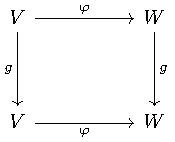
\includegraphics{figures/week-1-diag-1}
\]
commutes for every $g\in G$. (We will call this a \emph{$G$-linear map}
when we want to distinguish it from an arbitrary linear map between the
vector spaces $V$ and $W$). We can then define $\Ker\varphi$,
$\Img\varphi$, and $\Coker\varphi$, which are also $G$-modules.

A \emph{subrepresentation} of a representation $V$ is a vector subspace $W$
of $V$ which is invariant under $G$. A representation $V$ is called
\emph{irreducible} if there is no proper nonzero invariant subspace $W$ of
$V$.

If $V$ and $W$ are representations, so are $V\oplus W$ and $V\otimes W$
with $g(v\otimes w)\coloneqq gv\otimes gw$. Moreover, the $n$th tensor
power $\bigotimes^nV$, the exterior power $\bigwedge^n V$ and symmetric
powers $\Sym^n V$ are subrepresentations of it. The dual $V^*=\Hom(V,\bbC)$
of $V$ is also a representation, though not in the most obvious way: We
want the two representations of $G$ with respect to the natural pairing
between $V$ and $V^*$, so that if $\rho\colon G\to\GL(V)$ is a
representation and $\rho^*\colon G\to\GL(V)$ is its dual, then we have
\begin{equation}
  \label{eq:1:relation-1}
  \langle \rho^*(g)(v^*),\rho(g)(v) \rangle=\langle v^*,v \rangle
\end{equation}
for all $g\in G$, $v\in V$, and $v^*\in V^*$. This in turn forces us to
define the dual representation by
\[
  \rho^*(g)\coloneqq\prescript{\rmt}{}{\rho}(g^{-1})\colon V^*\longrightarrow V^*
\]
for all $g\in G$.

\begin{exercise}
Let us verify that \eqref{eq:1:relation-1} is satisfied by the definition
of $\rho^*$.
\end{exercise}
\begin{proof}
With $\rho^*$ as defined above, choose $g\in G$, $v\in V$ and $v^*\in
V$. Then, we have
\begin{align*}
  \langle \rho^*(g)(v^*),\rho(g)(v) \rangle=\langle v^*,v \rangle
  &=\langle  \rangle\\
  &=
\end{align*}
\end{proof}

Having defined the dual representation of the tensor product of two
representations, it is likewise the case that if $V$ and $W$ are
representations, then $\Hom(V,W)$ is also a representation, via the
identification $\Hom(V,W)=V^*\otimes W$. Unraveling this, if we view an
element of $\Hom(V,W)$ as a linear map $\varphi$ from $V$ to $W$, we have
\[
(g\varphi)(v)=g\varphi(g^{-1}v)
\]
for all $v\in V$. In other words, the definition is such that the diagram
\[
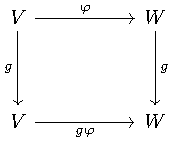
\includegraphics{figures/week-1-diag-2}
\]
commutes. Note that the dual representation is, in turn, a special case of
this: When $W=\bbC$ is the trivial representation, i.e., $gw=w$ for all
$w\in\bbC$, this makes $V^*$ into a $G$-module, with
$g\varphi(v)=\varphi(g^{-1}v)$, i.e.,
$g\varphi=\prescript{\rmt}{}{(g^{-1})}$.

\begin{exercise}
We verify that in general the vector space of $G$-linear maps between two
representations $V$ and $W$ of $G$ is just the subspace $\Hom(V,W)^G$ of
elements of $\Hom(V,G)$ fixed under the action of $G$. We will often denote
this space by $\Hom_G(V,W)$.
\end{exercise}
\begin{proof}
\end{proof}

We have taken the identification $\Hom(V,W)=V^*\otimes W$ as the
definition of the representation $\Hom(V,W)$. More generally, the usual
identities for vector spaces are also true for representations, e.g.,
\begin{align*}
V\otimes(U\oplus W)&=(V\otimes U)\oplus(V\otimes W)\\
\bigwedge^k(V\oplus W)&=\bigoplus_{a+b=k}{\textstyle\bigwedge^a V\otimes\bigwedge^b
  W}\\
{\textstyle\bigwedge^k V^*}&=\left({\textstyle{\bigwedge^kV}}\right)^*
\end{align*}

%%% Local Variables:
%%% mode: latex
%%% TeX-master: "../MA598-Lie-Groups"
%%% End:
